\chapter{Fejlesztői dokumentáció}
\label{ch:impl}

A szoftver működésének részletezéséhez elengedhetetlen a membránrendszerek formális modelljének ismerete, hiszen ezen rendszerek sajátos viselkedése az architechturális kérdésekben döntő szerepet képez.

A teljes definíció előtt azonban érdemes még pár fogalmat bevezetni. Általánosan tehát egy olyan absztrakt számítási modell áll a szoftver központjában, amely egy biológiai sejthez hasonló felépítéssel rendelkezik, ahol az egymásba ágyazott membránok régiókat különítenek el, amely régiókban különböző objektumok helyezkedhetnek el. A rendszerben az objektumokon felül szabályokat is rendelhetünk régiókhoz, ezen szabályok felelősek a membránrendszer állapotában végbemenő változásokért. A szabályokat a megfelelő feltételek teljesülése esetén kötelesek vagyunk alkalmazni, így egy evolúciós lépés a rendszer számításában addig tart, amíg van legalább egy akalmazható szabály. Érdemes már megjegyezni, hogy egy régió beazonosításához egy egyedi azonosítóra van szükség, illetve, hogy egy régiót könnyen azonosítani lehet az őt legszűkebben tartalmazó membránnal. Így természetes módon adódik, hogy a régiókat fa struktúrába tudjuk szervezni, amelyben minden egyes csúcs egy egyedi azonosítóval rendelkezik. Ezen fában a levelek az elemi membránokat reprezentálják, azaz azokat a régiókat, amelyeken belül nem helyezkedik el régió.  Ezen struktúra pedig nagyon könnyen megfeleltethető egy sztringnek.

A másik fontos tervezési szempont az objektumok reprezentálásához kapcsolódik. A membránrendszerek az egy régión belül megtalálható objektumok sokaságát ún. \textit{multihalmazokkal} reprezentálják, amelyben minden objektum rendelkezik egy multiplicitás értékkel, amely annak számosságát mutatja meg a régión belül. A multihalmaz teljeskörű értelmezéséhez pedig szükség van egy ábécére, amely a lehetségesen előforduló objektumok halmazát tartalmazza. Ezen multihalmazok felett pedig műveleteket kell tudni értelmezni, amelyek az evolúciós szabályok által megkövetelt funkciókat kell magukba foglalniuk. Mivel egy evolúciós szabály felhasználja az alkalmazásához szükséges objektumokat (azaz szintén egy multihalmazt), ezért szükség van egy olyan műveletre, amely a régióhoz tartozó multihalmazból eltávolítja a felhasznált objektumokat. Ezt a funkciót a multihalmazok közötti kivonás művelet fogja biztosítani. Ahhoz, hogy eldöntsük, hogy egy szabály alkalmazható-e egy régióban, elegendő megvizsgálni, hogy a régióhoz tartozó multihalmaz magába foglalja-e a szabályhoz tartozó bal oldali objektumok multihalmazát. Erre a problémára a halmazok közötti részhalmaz reláció nyújt megoldást. Végül az újonnan keletkező objektumokból álló multihalmaz hozzáadását a régió jelenlegi tartalmához a multihalmazokra nézett unió művelettel lehet modellezni. 

Ezen megjegyzések után már bevezethetjük a membránrendszerek formális definícióját \cite{tichler_slides}.

\section{Definíciók, formális modell}

\begin{definition}
Egy $\Pi = \langle O, \mu , \omega_1 , \dots , \omega_m, R_1 , \dots , R_m , i_o  \rangle$ rendezett $(2m + 3)$-ast membránrendszernek  nevezzük, ha

\begin{enumerate}
\item O egy objektumokból álló ábécé
\item $\mu$ egy \textit{m} membránból álló membránstruktúra. A régiók ekkor a $\{1,2, \dots, m\}$ elemeivel injektív módon vannak címkézve. Ilyenkor \textit{m}-et $\Pi$ \textit{fokának} nevezzük.

\item  $\omega_1 , \dots , \omega_m$ O feletti multihalmazokat reprezentáló sztringek, amelyek rendre az $1, 2, \dots, m$ címkéjű régiókhoz vannak rendelve

\item $R_i, 1 \leq i \leq m \; \mu \; i$-edik membránjához rendelt O feletti \textit{evolúciós szabályok} véges halmaza. A szabályok $u \rightarrow v$ alakúak, ahol $u \in O^+, v \in (O \times TAR)^*$, ahol $TAR=\{here, out\} \cup \{ in_j | 1  \leq j \leq m \} $ Ha nem írjuk ki a $j$ indexet, akkor nemdeterminisztikusan történik régió kiválasztása

\item$ i_o \in \{1,2, \dots, m\}$ egy elemi membrán címkéje, amely a modell kimeneti membránja.
\end{enumerate}
\end{definition}

Az előbbi definícióban meghatározott membránrendszerre a dolgozatban alapmodellként fogok hivatkozni. Az alkalmazás az alapmodell esetén csak a nemdeterminisztikus $in$ címkét engedi meg a szabályoknál. Ennek oka, hogy a szöveges reprezentációban csak így garantálható az, hogy egy karakter egy objektumot reprezentál, bárhol is szerepeljen a sztringben, illetve a régiók kézzel történő felcímkézésére sincs ezáltal szükség, hiszen ez lenne az egyetlen művelet, amely explicit használja a címkéket. 

A számítás formalizálásához fontos bevezetni a konfiguráció fogalmát.
\begin{definition}\label{def:mem_sysm}
A $C = (w_1, \dots, w_m)  \; a  \; \Pi = \langle O, \mu , \omega_1 , \dots , \omega_m, R_1 , \dots , R_m , i_o  \rangle$ membránrendszer konfigurációja, ha $w_i \in O^*$ és $w_i$ az $i$-edik régióban lévő objektumokból álló multihalmaz sztring reprezentációja
\end{definition}

\begin{note}
Egy $C$ konfiguráció kezdőkonfiguráció, ha $ \; \forall 1 \leq i \leq m$ esetén $w_i = \omega_i$
\end{note}

\begin{definition}
A megállási konfiguráció olyan konfiguráció, amelyre nem lehet már evolúciós szabályt alkalmazni.
\end{definition}

\begin{definition}
Az egylépéses konfigurációátmenet $C_1 \Longrightarrow_\Pi C_2$, akkor ha $C_1$-ből (a maximális párhuzamosság elvének megfelelve) egy evolúciós ütemben megkapható $C_2$ . 
\end{definition}

\begin{note}
Mivel a szabályok alkalmazása nemdeterminisztikus, ezért a konfigurációátmenet relációban egy $C_1$-hez több $C_2$ is létezhet.
\end{note}

\begin{definition}
A többlépéses konfigurációátmenet a $\Longrightarrow_\Pi$ reláció reflexív tranzitív lezártja. 
\end{definition}

A rendszer egy számítása alatt tehát a kezdőkonfigurációból egy megállási konfigurációba történő többlépéses konfigurációátmenet-sorozatot értünk.

\begin{note}
Ilyenkor a számítás eredményét többféleképpen definiálhatjuk. Alapértelmezetten a kimeneti régióban lévő objektumok számát jelenti. Az alkalmazás az alapmodell esetén ettől eltér és a környezetbe kijutó objektumok számát tekinti a számítás eredményének.
\end{note}

Létezik olyan kiterjesztése a(z) \ref{def:mem_sysm}. definíciónak, amelyben megengedünk olyan $u \rightarrow v \delta$ alakú szabályokat, ahol az $u \rightarrow v$ az eddigiekhez hasonló evolúciós szabály, a $\delta$ pedig egy speciális szimbólum, amely a membrán feloldódását jelzi a szabály alkalmazásának hatására. Tehát ha egy evolúciós lépésben alkalmazásra kerül egy ilyen speciális szabály, akkor az ütem végén a szabályhoz tartozó régió felbomlik, ilyenkor a benne lévő objektumok és membránok (a szabályok nem) a membránt közvetlenül tartalmazó szülő régióba kerülnek. A legkülső régió sosem oldódhat fel. 

A másik kiterjesztés a szabályok feletti részbenrendezés lehetőségét adja meg, mely szerint ha $r_1$ és $r_2$ relációban állnak (amelyet jelölhetünk $r_1 < r_2$-vel), akkor csak abban az esetben alkalmazható az $r_1$ szabály, ha $r_2$ már nem alkalmazható az evolúciós lépésben.

A szoftver mindkét kiterjesztést alapértelmezetten támogatja, működésükről a későbbi fejezetekben részletesebben szó esik.

Az alkalmazás az alapmodell mellett a szimport-antiport rendszerek szimulálását támogatja. 
Ebben a modellben az objektumok nem alakulhatnak át, csak a membránstruktúrán belül és a környezetbe vándorolhatnak. Az eddig definiált fogalmak a szimport-antiport rendszereknél is helyt állnak, egyedül a szabályok alakja és működése igényel módosításokat. 
Ezen felül a szimport-antiport rendszerek környezete rendelkezhet az $O$ ábécé egy olyan speciális részhalmazával, amelyben előforduló objektumok korlátlanul rendelkezésre állnak az evolúciós lépések során.
Ennek megfelelően vezessük be az alábbi definíciót.

\begin{definition}
Egy $\Pi = \langle O, \mu , E, \omega_1 , \dots , \omega_m, R_1 , \dots , R_m , i_o  \rangle$ rendezett $(2m + 4)$-est szimport-antiport rendszernek nevezünk, ha

\begin{enumerate}
\item O egy objektumokból álló ábécé
\item $\mu$ egy \textit{m} membránból álló membránstruktúra. A régiók ekkor a $\{1,2, \dots, m\}$ elemeivel injektív módon vannak címkézve. Ilyenkor \textit{m}-et $\Pi$ fokának nevezzük.

\item  $\omega_1 , \dots , \omega_m$ O feletti multihalmazokat reprezentáló sztringek, amelyek rendre az $1, 2, \dots, m$ címkéjű régiókhoz vannak rendelve

\item $E \subset O$ a környezetben korlátlanul rendelkezésre álló objektumok halmaza

\item $R_i, 1 \leq i \leq m \; \mu \; i$-edik membránjához rendelt O feletti szimport/antiport szabályok véges halmaza

\item$ i_o \in \{1,2, \dots, m\}$ egy elemi membrán címkéje, amely a modell kimeneti membránja.
\end{enumerate}
\end{definition}

Ebben a modellben legyenek $x, y \in O^+$ objektumok multihalmazait reprezentáló sztringek. A velük alkotott szabályok az alábbi alakok egyikét ölthetik:

\begin{enumerate}
\item (x, in): Ilyenkor az \textit{x} multihalmaz a membrán körül elhelyezkedő, őt legszűkebben tartalmazó régióból a membrán által határolt régióba vándorol
\item (x, out): Ilyenkor az \textit{x} multihalmaz az őt tartalmazó régióból a membránt körülvevő régióba mozog
\item (x, in; y, out): Ilyenkor az \textit{x} multihalmaz a membrán körül elhelyezkedő, őt legszűkebben tartalmazó régióból a membrán által határolt régióba vándorol, illetve az \textit{y} multihalmaz a szabályt tartalmazó régióból a membránt körülvevő régióba mozog
\end{enumerate}

Az első két szabályt \textit{szimport szabálynak}, míg az utolsót \textit{antiport szabálynak} nevezzük.

\begin{note}
Ezen két típuson kívül léteznek még $uniport$ szabályok is, amelyek felfoghatók olyan speciális szimport szabályként, amelyekben $|x| = 1$, ahol $|x|$ a multihalmazban szereplő objektumot számát jelöli.
\end{note}

A konfigurációkkal kapcsolatos definíciók megegyeznek az alapmodellben leírtakkal, kiegészítve azt a környezet $O-E$-beli objektumaiból álló $\omega_0$ kezdeti multihalmazt reprezentáló sztringgel, a későbbi konfigurációkban pedig $w_0$-val.


\section{Tervezés}

A feladat modellezésének legelső mozzanata az alkalmazáshoz szükséges osztályok meghatározása. Elsőként megállapítható, hogy a membránrendszerek egyes típusainak sok közös vonása van, ezért célszerű az absztrakt ősosztály \verb|MembraneSystem| bevezetése . Ez az osztály magába foglal olyan műveleteket, amelyeket minden szimulálandó membránrendszer köteles implementálni. Ez az osztály a kód karbantarthatóságát és bővíthetőségét is elősegíti, hiszen esetleges újabb membránrendszerek bevezetése esetén elegendő ezen osztály absztrakt metódusait implementálni. A szoftver esetében két konkrét membránrendszer típusról beszélhetünk, az alapmodellről (\verb|BaseModel|), illetve a szimport-antiport (\verb|SymportAntiport|)  rendszerekről, amelyek az ősosztály leszármazottaiként vannak jelen az osztály diagramban. 

Általánosan a membránrendszerek régiókból állnak, ezért a \verb|MembraneSystem| osztály az egy régiót reprezentáló \verb|Region| osztályból álló gyűjteményt komponál.  A két osztály közötti kapcsolat kompozíció, mivel egy membránrendszer nem létezne régiók nélkül, illetve absztrakt tekintetben egy régió sem létezhet önállóan, hanem egy csak egy komplexebb entitás (eukarióta sejt) részeként. Ezen régiók pedig valamilyen struktúrába szerveződve helyezkednek el a rendszerben, ennek eltárolására és karbantartására elhivatott a \verb|MembraneStructure| osztály, amely a \verb|Node| osztály segítségével egy \textit{n-áris} fát tárol el és a fa bejárásával begyűjti a membránrendszer által igényelt információkat. A régiók jelentős szerepet játszanak a membránrendszer szimulációjában, hiszen a bennük lévő objektumok és szabályok együttesen határozzák meg a generált nyelvet. Az osztály diagramban ennek megfelelően a \verb|Region| osztály  az objektumok multihalmazát reprezentáló \verb|MultiSet| osztályt és a szabályokat jelölő absztrakt \verb|Rule| osztályból álló gyűjteményt tartalmazza.
A szabályokat összefoglaló ősosztályból a konkrét típusokhoz tartozó szabályok származnak le, így az alapmodell esetén \verb|BaseModelRule| osztály képviseli a létrehozható szabályokat, míg a szimport-antiport rendszer esetében a \verb|SymportRule| látja el ezt a feladatot. Az alapmodellben tovább lehet specializálni a szabályokat, hiszen megadhatóak olyan szabályok, amelyek hatására a hozzá tartozó régió felbomlik, ezen funkciót a \verb|DissolvingRule| tölti be, amely a \verb|BaseModelRule|-ból származik le. A másik ilyen kiegészítése az alapmodellnek a szabályok közötti prioritási sorrend lehetősége, amely a \verb|PriorityRule| osztályban aggregált két \verb|BaseModelRule| típusú objektum segítségével éri el a kívánt viselkedést. A szabályok konstruáláskor valahogyan jelezni kell, hogy a kijelölt objektumokat reprezentáló multihalmaz milyen irányultsággal rendelkezik, azaz a szabály alkalmazása után melyik régióba fog kerülni vagy esetleg kijut a környezetbe. Ezt az információt az alapmodellbeli szabályok esetén a \verb|Direction|, szimport-antiport rendszerek esetében pedig a TransportationRuleType  (enum) osztály hordozza.
Jegyezzük meg, hogy nem csak egy régió hordozhat objektumokat, hanem a membránrendszer környezete is, amely tartalmazhat (akár korlátlan mennyiségben is) objektumokat. Ezért a membránrendszer a régiókon felül a \verb|Environment| osztályt is komponálja, amely számon tartja a környezetben korlátlan számban rendelkezésre álló objektumok és a kijutó objektumok multihalmazát.


\subsection{Architektúra}
Az alkalmazás a \textit{modell/nézet} architektúra elveit követve készült el, ahol a felhasználó mindig a grafikus felhasználói felülettel (nézet) lép interakcióba, amelynek hatására a modell és a nézet közötti kommunikáció eredményeképpen történik változás az alkalmazás állapotában.

A szoftverhez használt eszközök és környezet:
\begin{itemize}
\item \textit{Python} programozási nyelv \textit{3.10.4}-es verzió, a \textit{PySide6} modul kiegészítésével
\item \textit{Qt} keretrendszer \textit{5.15.3}-as verzió
\end{itemize}

\section{Modell}

\begin{figure}[H]
\advance\leftskip-3cm
	\scalebox{0.75}[0.75]{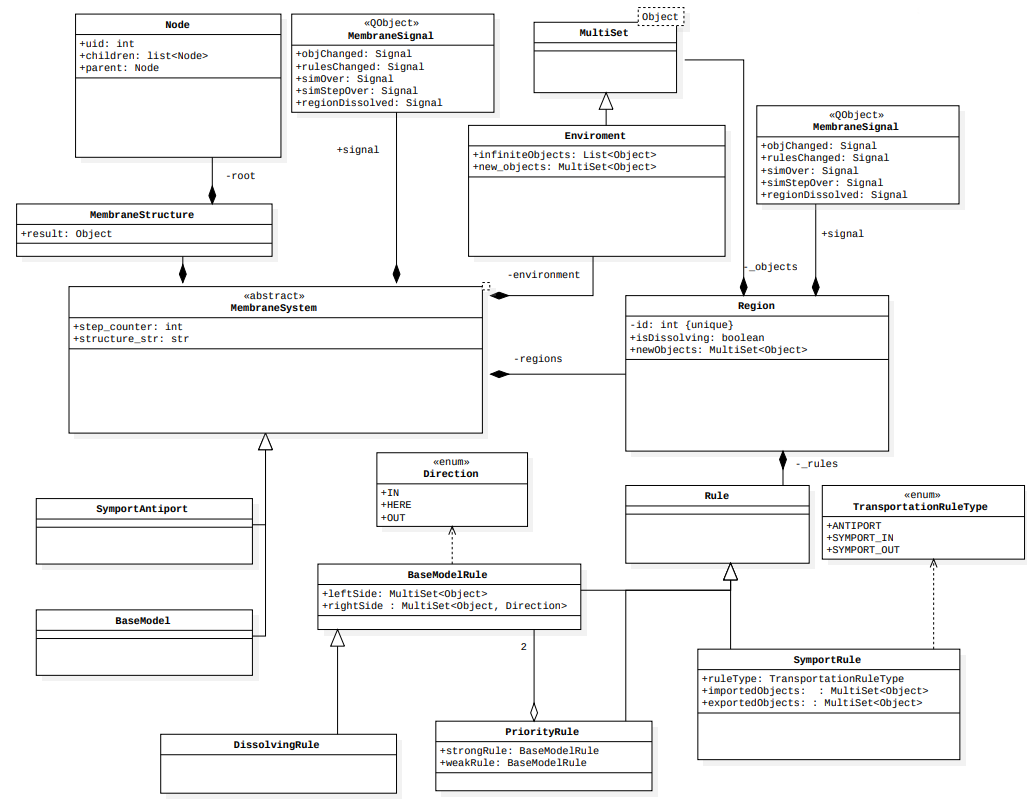
\includegraphics{model_uml_no_methods.png}}
	\caption{A modell osztálydiagramja}
	\label{fig:model_no_methods}
\end{figure}

A \ref{fig:model_no_methods} ábra mutatja az osztálydiagramot, amelyben még nem szerepelnek az osztályszintű- és példánymetódusok. Az eddig említett osztályokon felül megjelenik két, a modell és a nézet közötti üzenetváltásért felelős, \verb|QObject|-ből leszármazó osztály, a \verb|MembraneSignal| és a \verb|RegionSignal| . Az előbbi a teljes membránrendszerben előforduló szignálokat küldi tovább a megjelenítésért felelős osztályoknak, míg az utóbbi az egyes régiók tartalmának megváltozását hivatott jelezni. A szoftver működéséhez szükséges osztályok meghatározása még nem elegendő céljának megvalósításához, ugyanis szükség van ezen osztályok metódusain keresztül a szimulálás folyamatának megtervezésére is.

\subsection{Objektumok}

Az objektumokat reprezentáló multihalmazokat a \verb|MultiSet| osztály segítségével hozhatjuk létre. Ezen osztály példányai felett értelmezve van az unió és a kivonás művelete, a részhalmaz reláció, illetve lekérdezhető egy tetszőleges objektum multiplicitása. A \verb|MultiSet| osztály kiemelt fontosságú a számítás során, hiszen egy szabály alkalmazhatóságának eldöntéséhez két multihalmaz (nevezetesen a régió objektumait tartalmazó és a szabály által megkövetelt objektumait tartalmazó) közötti részhalmaz reláció eldöntésére van szükség. Ha valóban alkalmazható egy szabály, akkor a szabály bal oldala felhasználásra kerül, tehát egy kivonás műveletet kell végezni, a létrejövő objektumok pedig a megfelelő régióhoz az unió műveletével tudnak hozzákerülni. Tehát az osztályt nem csak a régiók, hanem a szabályok is felhasználják működésük során.

\begin{figure}[H]
\centering
	\scalebox{0.75}[0.75]{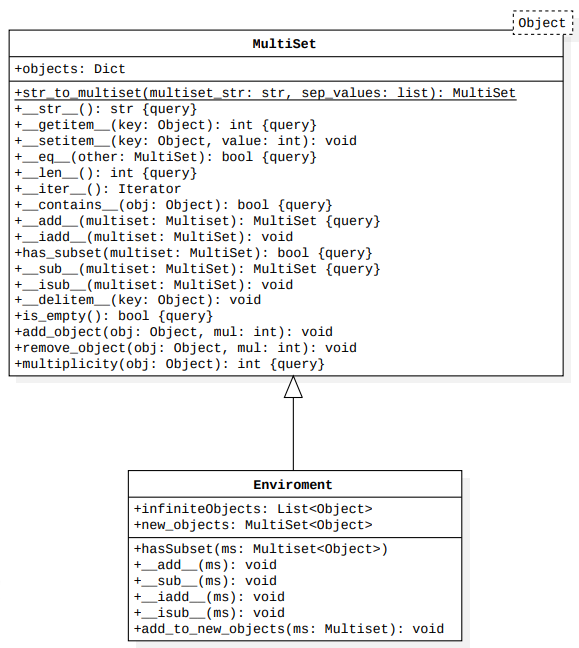
\includegraphics{multiset_class.png}}
	\caption{Az objektumokat reprezentáló multihalmaz és a környezet \textit{UML} diagramja}
	\label{fig:multiset_uml}
\end{figure}

A környezet reprezentálására hivatott \verb|Environment| osztály a korlátlanul rendelkezésre álló objektumokat tartalmazó \verb|infinite_obj| listával egészíti ki a \verb|MultiSet| osztályt, illetve az ősosztályban használt műveletek is felüldefiniálja a helyes viselkedés érdekében. Mivel a környezet is \verb|MultiSet| típusú, ezért a dinamikus típusosság következtében az unió műveletet meghívhatnánk rá \verb|MultiSet| típusú paraméterrel, ennek eredménye szintén \verb|MultiSet| típusú lenne (ami a környezet aktualizálásakor egy evolúciós lépésben nem lenne szerencsés). Ennek elkerülése érdekében ezen műveleteket implementáció nélkül felüldefiniálja az osztály és csak olyan műveletet biztosít, amely a metódushoz tartozó (\verb|self|)  példányhoz unió művelet segítségével hozzáad egy multihalmazt. A hozzáadás során az \verb|infinite_obj|-ban megtalálható objektumok figyelmen kívül hagyhatók. A kivonás esetén is hasonlóan járunk el, illetve ha speciálisan olyan objektumot kell levonni, amely korlátlan számban áll rendelkezésre, olyankor az mellékhatás nélkül végrehajtódhat.

\subsection{Membránstruktúra}

Mivel a membránrendszer struktúrája egyes típusok esetében módosulhat, ezért fontos, hogy a rendszer szerkezete ne statikusan legyen tárolva, hanem a membránrendszer megkonstruálása után is dinamikusan tudjon változni.  Ezeket az elvárásoknak megfelelő \textit{n}-áris fát láncolt lista adatszerkezettel kerül megvalósításra, amelynek fejelemét (fák esetén inkább gyökerét)  a \verb|MembraneStructure| osztály adattagként tárolja el. Minden csúcs egyedi azonosítóval rendelkezik, amely megegyezik a hozzátartozó régió címkéjével. Emellett minden csúcs számontartja a saját szülőjét, illetve gyermekeiből álló \verb|children| listát, amelyhez az \verb|add_child| metódussal lehet új elemet fűzni. Az osztály többi művelete \textit{getter} vagy \textit{setter} metódusként funkcionál.

\begin{figure}[H]
\centering
	\scalebox{0.75}[0.75]{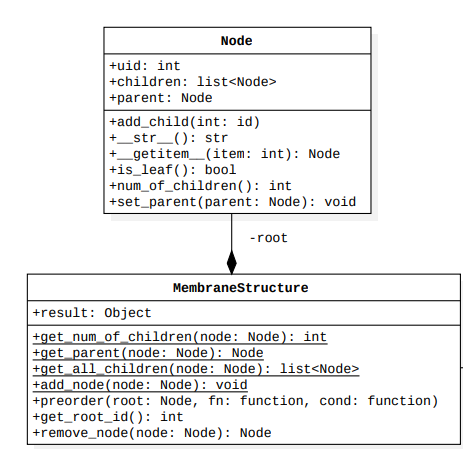
\includegraphics{node_and_structure_class.png}}
	\caption{A membránrendszer struktúrájáért felelős osztályok}
	\label{fig:node_and_structure_uml}
\end{figure}


A \verb|MembraneStructure| osztály a fa struktúra karbantartásáért és a struktúrával kapcsolatos ,,lekérdezésekért'' felelős. Ezen feladatok ellátásához kulcsszerepet kap a \verb|preorder(root, fn, cond)| metódus, amely a bejárja a fát és ha egy \textit{n} csúcsra teljesül a \verb|cond| függvény feltétele, akkor az  \verb|fn| függvény kerül meghívásra.

\lstset{caption={Membránstruktúra preorder bejárása}, label=src:preorder}
\begin{lstlisting}[language={Python}]
def preorder(self, root, fn, cond):
        if root is None:
            return
        if cond(root):
            self.result = fn(root)
        else:
            iter_count = root.num_of_children()
            for i in range(iter_count):
                self.preorder(root.children[i], fn, cond)
\end{lstlisting}

A \verb|MembraneStructure| kialakítása igazodik ehhez a szemantikához, mivel mind a négy osztályszintű metódus és a \verb|remove_node()| metódus is egy \verb|Node| típusú paramétert vár, amelyen végrehajtják a kívánt műveletet. Tehát ezen metódusok nem járják be a fát és keresik meg a megfelelő címkéjű csúcsot, hanem a \verb|preorder| függvény paramétereként kerülnek felhasználásra, amelyben a feltétel a csúcs egyedi azonosítójára szűr. Mivel a rekurzív függvénynek tetszőleges típusú visszatérési értéke lehetne, ezért a visszaadandó érték a struktúra \verb|result| adattagjába kerül. Az osztály felépítése garantálja, hogy a result lekérdezései nem keresztezhetik egymást, ezáltal elkerülve az inkonzisztens és helytelen eredményeket.

\subsection{Szabályok}

A szabályok a membránrendszer számításaiban központi szerepet kapnak, ám kevés olyan tulajdonságuk van, amely minden típusban közös vonásként jelenik meg. Ezért az absztrakt \verb|Rule| ősosztály kevés implementálandó metódust határoz meg, csak a szabályhoz tartozó szöveges reprezentáció, illetve a szabály súlyát meghatározó műveletek meglétét írja elő. 


\begin{figure}[H]
\centering
	\scalebox{0.6}[0.6]{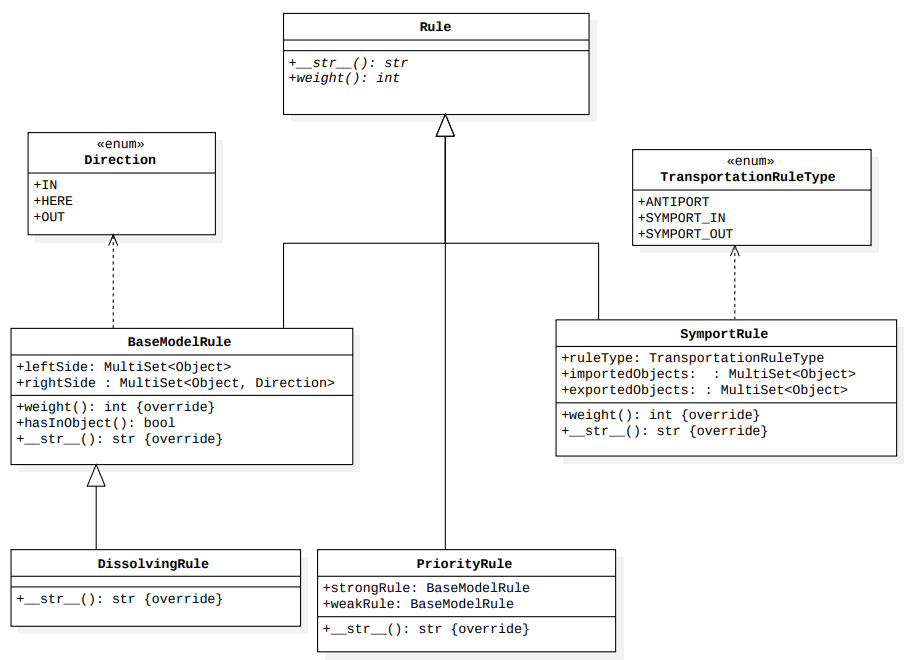
\includegraphics{uml_rule_class.png}}
	\caption{A membránrendszer szabályait modellező osztályok}
	\label{fig:rule_uml}
\end{figure}

Az alapmodellhez tartozó \verb|BaseModelRule| osztály a leszármazás mellett rögzíti a modellezéséhez szükséges két adattagot. Az egyik a \verb|left_side|, amely a szabály végbemeneteléhez szükséges objektumokból álló multihalmazt tárolja (\verb|objektum-multiplicitás| párok formájában), a másik pedig a \verb|right_side|, amely a szabály alkalmazásának következtében létrejövő objektumokat és azok mozgásának irányát adja meg. Ezen irányok jelzésére a \verb|Direction| osztályban rögzített \verb|HERE|, \verb|IN| és \verb|OUT| felsorolási típus értékei hivatottak. Tehát a \verb|right_side| olyan multihalmazban a megfelelő multiplicitással \verb|(objektum, irány)| párok szerepelnek.
Tehát egy evolúciós lépésben az alapmodellbeli szabály alkalmazhatóságának eldöntése a szabály bal oldala és a régióhoz tartozó objektumokból álló multihalmaz közötti tartalmazási reláció vizsgálatával ellenőrizhető. 
Az alapmodell kiegészítéseként beszélhetünk a feloldódás fogalmáról, amely a modellezés során a \verb|BaseModelRule|-ból leszármaztatott \verb|DissolvingRule| osztály segítségével kerül megvalósításra. Ez az osztály semmilyen új metódust vagy adattagot nem vesz fel, az információtartalom a példányosítása mögött rejlik, hiszen ilyen típusú szabály alkalmazása az adott régió \verb|is_dissolving| adattagjának igaz értékre billentését idézi elő. 
Az alapmodell másik ilyen kiterjesztése a szabályok közötti részbenrendezés lehetőségét nyújtja, amelyet az alkalmazás két szabály közötti prioritás rögzítésével támogatja. Az ilyen szabályok közötti relációk leírására a \verb|PriorityRule| szolgál, amely létrehozásakor két alapmodelli szabályt vár paraméterül.
Egy \verb|PriorityRule| típusú szabály alkalmazhatóságának vizsgálata során először a nagyobb prioritással rendelkezdő szabály alkalmazhatóságát kell vizsgálni, majd annak esetleges  sikertelensége esetén lehet a kisebb prioritással rendelkező szabály alkalmazhatóságát elemezni.

A szimport-antiport rendszerek esetében a bal-és jobb oldali objektumok helyett \textit{importált} és \textit{exportált} objektumok multihalmazáról beszélhetünk, ahol új objektumok nem jöhetnek létre, csak régiók között vándorolhatnak. Attól függően, hogy ezen két interakció közül melyek hajtódnak végre egy szabályban, három különböző szabálytípust lehet megkülönböztetni, amelyek jelzésére a \verb|TransportationRuleType| felsorolási típus értékei hivatottak. Ezek pedig rendre:
\begin{compactenum}
\item \verb|SYMPORT_IN|
\item \verb|SYMPORT_OUT|
\item \verb|ANTIPORT|
\end{compactenum}

\subsection{Régiók}

\begin{figure}[H]
\centering
	\scalebox{0.6}[0.6]{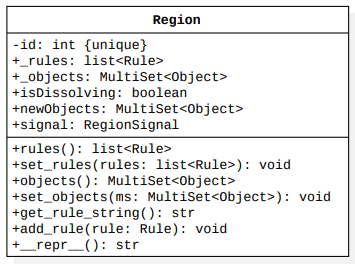
\includegraphics{uml_region_class.png}}
	\caption{A membránrendszer régióit reprezentáló osztály}
	\label{fig:region_uml}
\end{figure}

Egy régió azonosítására a saját egyedi azonosítóját (\verb|id|) használja az alkalmazás, amely megegyezik a membránstruktúrában a hozzá tartozó \verb|Node| objektum \verb|uid| adattagjában tárolt értékkel. Ez az érték a rendszer számítása során nem változik, egyedül egy régió szülőjének címkéje változhat meg (alapmodell esetén feloldódás következtében), ezért ezt az értéket nem lehet statikusan letárolni. A feloldódás jelzésére az \verb|is_dissolving| adattag hivatott, amelynek igaz értékre billenése esetén az evolúciós lépés végén a régió felbomlik. A régió emellett felveszi a \verb|new_objects| adattagot is, amely azon objektumok eltárolására szolgál, amelyek az éppen zajló evolúciós lépésben kerültek a régióba. Ez azért fontos, mert a maximális párhuzamosság elve szerinti szabályok kiválasztása egyidejűleg történik meg az ütem elején, tehát az egyik szabály alkalmazásának mellékhatása nem befolyásolhatja a kiválasztott szabályokat. Ezért amikor alkalmazásra kerül egy szabály, a jobb oldalán található objektumok elrejtésre kerülnek a további szabályok elől, majd az evolúciós lépésben a maximális szabálymultihalmaz szelektálása után kerülnek a régió \verb|objects| multihalmazába. 

\subsection{Membránrendszer ősosztály és leszármazottai}

Az absztrakt membránrendszer ősosztály az eddig taglalt osztályok segítségével képes sablont nyújtani a számítás modellezéséhez. A \verb|MembraneSystem| nem példányosítható (mivel tartalmaz absztakt metódusokat), de konstruktorában a rendszer régiót tartalmazó gyűjteményt, a membránstruktúrát reprezentáló \verb|MembraneStrucutre| objektumot várja paraméterül. A régiókat egy olyan asszociatív tömbben tárolja el a membránrendszer, amelyben a kulcs a régió azonosítója, a hozzá tartozó érték pedig a régió objektum.A leszármaztatott \verb|BaseModel| és \verb|SymportAntiport| osztályok megöröklik ezt a konstruktort, amelyet a saját konstruktorukban meghívnak. A szimport-antiport rendszerek esetében még a kimeneti régió címkéjét is meg kell adni, ezért ott az további paraméterként jelenik meg. Alapmodell esetében az alkalmazás a környezetbe kijutó objektumok számát tekinti eredménynek, ezért ott nincs szükség további specifikálásra. 

\begin{figure}[H]
\centering
\advance\leftskip-3.5cm
	\scalebox{0.6}[0.6]{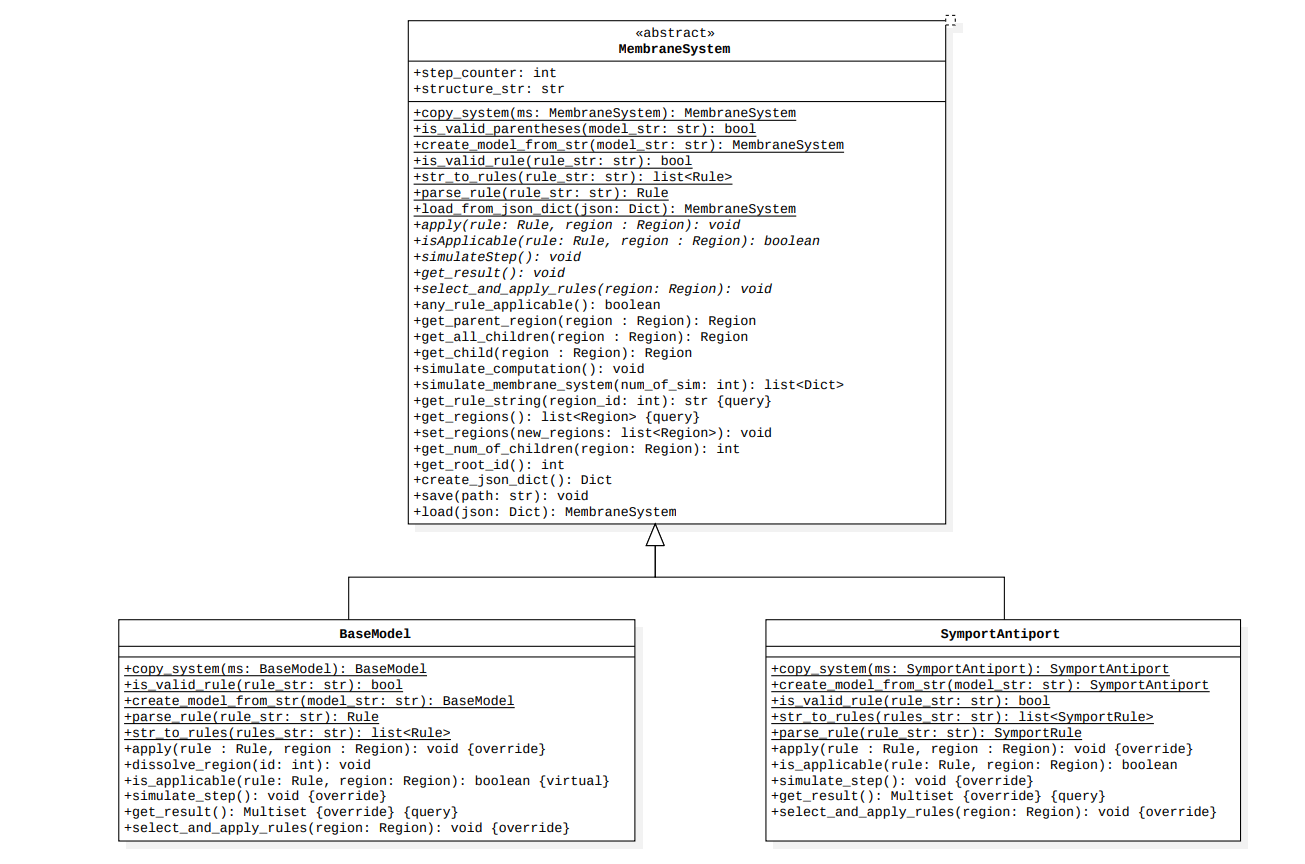
\includegraphics{uml_membrane_systems_class.png}}
	\caption{A membránrendszert modellező absztrakt osztály és leszármazottai}
	\label{fig:system_uml}
\end{figure}

A \verb|MembraneSystem| implementálja a membránrendszer felépítésével kapcsolatos lekérdezéseket. Így például a \verb|get_parent_region()| metódus a paraméterként kapott régió szülő régióját adja vissza. 
A megvalósításnál a \verb|MembraneStructure| osztály \verb|preorder()| metódusát használja fel, amely a fa gyökeréből indítva a megfelelő \verb|MembraneStructure| osztályszintű metódusával kiegészítve a kívánt viselkedést eredményezi.

\newpage

\lstset{caption={Szülő régió lekérdezése}, label=src:get_parent}
\begin{lstlisting}[language={Python}]
def get_parent_region(self, region):
        region_id = region.id
        self.tree.preorder(self.tree.skin, self.tree.get_parent,
                           lambda x: x.id == region_id)
        result_node = self.tree.result
        return self.regions[result_node.id]
\end{lstlisting}


Ez a lekérdezés akkor kerül használatra, amikor egy szabály jobb oldalán  \verb|OUT| címkéjű objektum található, ugyanis ilyenkor a szülő régióba fog kerülni az evolúciós lépés során. Ezt a felépítést követi a többi struktúrával kapcsolatos metódus is.

\subsection{Számítás algoritmusa}

Ezen metódusok segítségével minden rendelkezésre áll ahhoz, hogy a membránrendszer számítását modellezni tudja a szoftver. Vannak olyan metódusok, amelyek a membránrendszerek definíciója szerint minden típusban meg kell, hogy egyezzenek. Ilyen például az, hogy mindegyik rendszer számításának kell legyen eredménye, illetve, hogy addig történnek a konfigurációátmenetek ameddig nem jut megállási konfigurációba. Tehát a \verb|MembraneSystem| osztályban bevezetésre kerülhet a \verb|simulate_computation()| metódus, amely megadja a számítás vázát. 

\lstset{caption={Membránrendszer számításának általános algoritmusa}, label=src:simulate_comp}
\begin{lstlisting}[language={Python}]
def simulate_computation(self):
	while self.any_rule_applicable():
     	self.simulate_step()
	return self.get_result()
\end{lstlisting}

A felhasznált metódusok közül csak a \verb|any_rule_applicable()| metódushoz rendelhető általános implementáció, a többi metódus eltérően viselkedhet a különböző típusok esetében. Tehát az \verb|any_rule_applicable()| metódus feladata, hogy megvizsgálja, hogy van-e alkalmazhazó szabály a rendszerben. Annyiszor fut le tehát szimulációs lépés, ahányszor ez a feltétel teljesül; ennek hiányában a megállási konfigurációba jutott állapotban az előre definiált eredményével tér vissza a metódus.

\lstset{caption={Membránrendszer leállási feltétel ellenőrzése}, label=src:any_rule_appl}
\begin{lstlisting}[language={Python}]
def any_rule_applicable(self):
	for region in self.regions.values():
		for rule in region.rules:
			if self.is_applicable(rule, region):
				return True
	return False
\end{lstlisting}

A metódus végigiterál az összes régión, azon belül a régió egyes szabályain, és ha talál egy alkalmazható szabályt az \verb|is_applicable()| metódus segítségével, akkor \textit{igaz} értékkel tér vissza, egyébként \textit{hamissal}.
Az \verb|is_applicable()| metódus viselkedése eltér az alapmodell és a szimport-antiport rendszerek esetében, ezért ehhez a metódushoz a \verb|MembraneSystem| osztályban nem tartozik implementáció.

Ezen kívül az absztrakt ősosztály több metódus vázát is tartalmazza, ilyen a szabály alkalmazását elvégző \verb|apply()| metódus és a szabályok nemdeterminisztikus kiválasztására szolgáló \verb|select_and_apply_rules()|.
Ezek után az alapmodell és szimport-antiport rendszerek sajátosságait figyelembe véve adható algoritmus a számítás leírásához.

\subsubsection{Alapmodell}

Az alapmodell esetén fontos megjegyezni, hogy a számítás nemdeterminisztikusságának garantálásához nem szükséges megengedni, hogy a szabályok kiválasztása a teljes membránrendszer egészére nézve történjen, hanem elegendő valamilyen sorrendben végighaladni a rendszer összes régióján és lokálisan nézve alkalmazkodni a maximális párhuzamosság elvének, hiszen az adott ütemen belül egy szabály alkalmazásának nincs kihatása egy másik régióra. Így a \verb|simulate_step()| metódus végigiterál a régiókon, és mindegyikre meghívja a \verb|select_and_apply_rules()| metódust. Miután az összes alkalmazható szabály végrehajtása megtörtént, utána történik az egyes régiók tartalmának frissítése. Ez azt jelenti, hogy az ütem során a \verb|new_objects| multihalmazba kerülő objektumok hozzáadódnak az \verb|objects| adattaghoz, majd a \verb|new_objects| tartalma üresre állítódik. A frissítés közben ellenőrzésre kerül, hogy egy régióban végbement-e egy feloldódást előidéző szabály, ugyanis ilyenkor meghívódik a \verb|dissolve_region()| metódus a szóban forgó régióra. 

A \verb|dissolve_region()| metódus feladata, hogy a felbomló régióban lévő objektumokat és egyéb régiókat a szülő régióhoz adja, illetve, hogy kitörölje a \verb|regions| asszociatív tömbből a régióhoz tartozó bejegyzést.
A \verb|select_and_apply_rules()| metódus feladata tehát egy adott régión belül a maximális párhuzamosság elvének megfelelve szabályok nemdeterminisztikus kiválasztása, amely kiválasztása után meghívja az adott szabályt (a kiválasztott régióra) az \verb|apply()| metódus segítségével.

\lstset{caption={Szabályok kiválasztása az alapmodell esetében}, label=src:base_select}
\begin{lstlisting}[language={Python}]
 def select_and_apply_rules(self, region):
        indices = list(range(len(region.rules)))
        while indices:
            idx = random.choice(indices)
            if self.is_applicable(region.rules[idx], region):
                self.apply(region.rules[idx], region)
            else:
                indices.remove(idx)	
\end{lstlisting}

A metódus minden régióbeli szabályhoz rendel egy sorszámot, amelyet az \verb|indices| listában elhelyez. Ebből a listából nemdeterminisztikusan választ egy elemet a beépített \verb|random.choice()| metódus segítségével, amely a listabeli elemek közül egyenletes eloszlás szerint választ. Ezután ha a kiválasztott szabály alkalmazható, akkor meghívja az \verb|apply()| metódust a kiválasztott indexhez tartozó szabállyal, ellenkező esetben pedig törli a sorszámot a listából. Ezen mechanizmus segítségével képes egy régión belül ugyanazon objektumok és szabályok esetén más végeredmény kialakulni. 
 
 A \verb|select_and_apply_rules()| metódus működéséhez szükség volt az \verb|is_applicable()| metódusra, amely egy adott szabályról eldönti, hogy alkalmazható-e a jelenlegi konfigurációban.
 Ez a metódus figyelembe veszi a paraméterben megkapott \verb|rule| változó dinamikus típusát és ez alapján határozza meg a visszatérési értékét. Ha ugyanis a paraméterben kapott változó típusa \verb|PriorityRule|, akkor azt kell megvizsgálnia, hogy a két szabály közül akárcsak az egyik alkalmazható-e, hiszen ez azt jelenti, hogy az erősebb vagy ha az erősebb nem, akkor a gyengébb szabály végrehajtható. Ezzel a \verb|PriorityRule| szabályok esetét a másik két típus esetére vissza lehet vezetni. A \verb|DissolvingRule| osztálybeli szabályok nem alkalmazhatóak a legkülső (skin) régióban. Ezek után a hátralévő két típusnál elegendő azt megvizsgálni, hogy a szabályhoz tartozó bal oldal részhalmaza-e a régió objektumainak (nem figyelembe véve az evolúciós lépés során újonnan bejutó objektumokat). 
 Ez a feltétel a \verb|region.objects.has_subset(rule.left_side)| metódushívással eldönthető, ahol a \verb|region.objects| az adott régió jelenlegi állapotához tartozó multihalmaz, a \verb|rule.left_side| pedig a vizsgált szabály bal oldala (amely szintén egy multihalmaz).

A teljes számítás modellezésének leírásához már csak az \verb|apply()| metódust kell definiálni. Az \verb|apply()| metódus meghívása csak olyan esetben történik meg, amikor a szabály alkalmazhatósága bebizonyosodott, ezért ez a függvényben nem kerül ellenőrzésre. A metódus feladata kivonni a szabály végrehajtásához szükséges objektumokat a régió objektumaiból, majd végigmenni a szabályhoz tartozó jobb oldalból álló multihalmazon és a megfelelő régió vagy környezet új objektumaiból álló multihalmazhoz hozzáadni a keletkező objektumokat. A szabály jobb oldala egy olyan multihalmaz, amelyben az értékek \verb|(objektum, irány)| párokból állnak. 
Az \verb|irány| alapján tehát lehet:
\begin{compactenum}
\item \verb|IN|: Ilyenkor az objektum az egyik véletlenszerűen kiválasztott gyerek régióba kerül (ilyen biztosan létezik).
\item \verb|OUT|: Ilyenkor az objektum szülő régióba vándorol. Ha a legkülső régióban kerül alkalmazásra ilyen szabály, akkor a környezethez jut. 
\item \verb|HERE|: Ilyenkor az objektum régión belül jön létre.
\end{compactenum}

Ha az alkalmazott szabály típusa \verb|DissolvingRule|, akkor a régió \verb|is_dissolving| adattagja \textit{igaz} értékre állítódik.

\subsubsection{Szimport-antiport rendszer}

Szimport-antiport rendszerek esetén nincs szó objektumok keletkezéséről, hiszen ebben a modellben az objektumok csak régiók között vándorolhatnak. Ebben a modellben viszont számít az, hogy régiónként milyen sorrendben választunk szabályokat, hiszen egy antiport típusú szabály a szülő régió objektumait is igényli végbemeneteléhez. 

% Erre egy példa ábra ha nem lenne elég oldal

Ennek következtében több metódusnál is más megközelítést kell alkalmazni. A \verb|select_and_apply_rules()| metódus globálisan fog szabályokat kiválasztani a teljes membránrendszert lefedve, ez garantálja a teljes nemdeterminisztikusságot ennél a modellnél.

\lstset{caption={Szabályok kiválasztása a szimport-antiport rendszer esetében}, label=src:symport_select}
\begin{lstlisting}[language={Python}]
def select_and_apply_rules(self):
	rule_indices = {}
	idx = 0
	for region in self.regions.values():
		for rule in region.rules:
			rule_indices[idx] = (rule, region)
			idx = idx + 1
	while rule_indices:
		rand_idx = random.choice(list(rule_indices.keys()))
		rand_rule = rule_indices[rand_idx][0]
		rand_region = rule_indices[rand_idx][1]
		if self.is_applicable(rand_rule, rand_region):
			self.apply(rand_rule, rand_region)
		else:
			del rule_indices[rand_idx]
\end{lstlisting}

A metódus elején a \verb|rule_indices| asszociatív tömb sorszám-szabály párosokkal kerül feltöltésre a membránrendszerben megtalálható összes régión keresztül történő iterálással. Ezek után az alapmodellhez hasonlóan nemdeterminisztikusan egy index kerül kiválasztásra, amelyhez tartozó szabály alkalmazhatóságát vizsgálja az \verb|is_applicable()| metódus. Amennyiben ez sikeres, a szabály végrehajtódik, egyébként törlődik a szótárból a hozzá tartozó bejegyzés.

A \verb|simulate_step()| metódusban az előbb említett \verb|select_and_apply_rules()| metódus meghívása után csak a régiók állapotának frissítése van hátra. Ilyenkor az alapmodellhez hasonlóan minden régióban és ebben az modellben a környezetben is a \verb|new_objects| multihalmaz tartalma hozzáadásra kerül az \verb|objects| multihalmazhoz, majd az előbbi kinullázásával befejeződött a szimulációs lépés. Emellett a metódus még eggyel megnöveli a lépések számát tartalmazó \verb|step_counter| adattag értékét.

Egy szabály alkalmazhatóságának kérdése szimport-antiport rendszerek esetében egy fokkal összetettebb, hiszen a környezet rendelkezhet korlátlan mennyiségben objektumokkal, amelyek külön vizsgálatatot igényelnek. Ezen speciális eseteken kívül minden alkalommal azt kell vizsgálni, hogy az exportált objektumokból álló multihalmaz részhalmaza-e a régióhoz tartozó objektumok multihalmazának és/vagy az importált objektumokból álló multihalmaz részhalmaza-e a szülő régiónak (esetlegesen a környezetnek).

Ha az \verb|is_applicable()| metódus úgy ítélte, hogy az adott régió egyik szabálya alkalmazható, akkor az \verb|apply()| metódus kerül meghívásra. Mindhárom szabálytípusnál ilyenkor újból meg kell vizsgálni, hogy a legkülső régióban történik-e a reakció, hiszen az importálásnál és az exportálásnál a korlátlan számban meglévő objektumok multiplicitásán nem kell módosítani. A többi esetben a beérkező objektumok a régió \verb|new_objects| multihalmazába kerülnek, a kijutó objektumok pedig a \verb|objects| multihalmazból kerülnek levonásra.


\subsection{Párhuzamos számítások}

Egy membránrendszer nemdeterminisztikussága miatt érdemes a kezdőkonfigurációból több szimulációt is indítani, hogy megfigyelhetőek legyenek az esetleges mintázatok a számítás folyamatában. Ezt a funkciók a \verb|MembraneSystem| osztály a \verb|simulate_parallel()| metóduson keresztül biztosítja. Ezen metódus meghívásakor előre meghatározott számú szimuláció indul el az aktuális membránrendszer konfigurációjából, ám ezek egymást semmilyen módon nem befolyásolják.

\lstset{caption={Párhuzamos szimulációt végrehajtó metódus}, label=src:compute_parallel}
\begin{lstlisting}[language={Python}]
def simulate_parallel(self, num_of_sim=100):
	def compute(model):
		model_copy = model.__class__.copy_system(model)
		model_copy.simulate_computation()
		return model_copy.get_result()

	cpu_count = multiprocessing.cpu_count()
	futures = []
	results = []
	with ThreadPoolExecutor(max_workers=cpu_count) as executor:
		for i in range(num_of_sim):
			futures.append(executor.submit(compute, self))
		for i in range(num_of_sim):
			results.append(futures[i].result())
	self.signal.sim_over.emit(results)
	return results
\end{lstlisting}

A párhuzamos számítások megkezdése előtt fontos, hogy lehessen másolatot készíteni a membránrendszerről. Mivel a Python nyelv alapértelmezetten referencia szerint másol le egy objektumot, a naiv másolás azt eredményezné, hogy a különböző számítások ugyanazon a membránrendszeren történnének, amely számos problémát előidézéséhez vezetne. A kívánt másolatokhoz létrehozásához mély másolást kell alkalmazni, amelyhez a \verb|copy| modul ad támogatást. A \verb|MembraneSystem| osztály abból következően, hogy leszármazik a \verb|QObject| osztályból, nem szerializálható. Emiatt a mély másolást a létrehozásához elengedhetetlen adattagokon keresztül kell megvalósítani.
Ehhez az absztakt ősosztályban definiált \verb|copy_system()| metódus az egyes leszármazott típusoknál való felüldefiniálással valósítható meg.

Tehát a \verb|compute()| metódus először készít az aktuális állapotról egy másolatot, majd arra meghívja a számítást végző \verb|simulate_computation()| metódust és visszatér annak eredményével.
Az egyes számítások egy \verb|ThreadPoolExecutor| osztály segítségével kerülnek külön logikai szálakra. A számítások feldolgozásának rendelkezésére álló szálak száma megegyezik a futtató számítógépben található processzormagok számával. A paraméterben megadott \verb|num_of_sim| változó hordozza az ismétlések számát, amellyel megegyező számú szál fog indulni. Az egyes szálakon elindított \verb|compute()| metódusok visszatérési értékeit a \verb|futures| listába elhelyezett \verb|Future| típusú objektumok fogják tartalmazni. Az \verb|executor.submit(compute, self)| metódus segítségével kiadjuk a metódus ütemezését a \verb|ThreadPoolExecutor| típusú \verb|executor| objektumnak. A \verb|result | listába ezek után elhelyezhetőek az eredmények, a \verb|futures[i].result()| metódushívással. Ez egy blokkoló művelet, tehát amíg nem tér vissza az \textit{i}-edik számítás, addig várakozik a vezérlési szál. Ezzel lehet garantálni, hogy a \verb|simulate_parallel()| metódus csak akkor tér vissza a \verb|results| listával, amikor már minden számítás befejeződött. 

\subsection{Mentés}
Az alkalmazás biztosítja egy membránrendszer lementését, ezért a modellnek támogatnia kell állapotának olyan formátumba való exportálását, amely alkalmas arra, hogy azt az állapotot vissza lehessen állítani. Ehhez kapcsolódóan fontos megjegyezni, hogy a felhasználó egy sztring megadásával is létrehozhat egy membránrendszert, amely rögzíti annak struktúráját és esetlegesen objektumait. Ezt a sztringet a modell inicializálásakor a \verb|structure_str| adattagjába lementi, hiszen az az algoritmus, amely a legelső alkalommal ebből előállítja a megfelelő típusú \verb|MembraneSystem| osztályból leszármazó objektumot, az az újbóli előállításnál is ugyanazon algoritmussal vissza tudja állítani ezt az állapotot. Viszont ez az állapot eltérhet az eredeti konstruálás pillanatától, objektumok és régiók hozzáadásának, illetve törlésének következtében. Ezért a lementés előtt ezt a kezdeti \verb|structure_str| változót módosítani kell. 	

\lstset{caption={Mentésért felelős metódus}, label=src:save_model}
\begin{lstlisting}[language={Python}]
def save(self, path):
	json_dict = self.create_json_dict()
	with open(path, 'w') as save_file:
		json.dump(json_dict, save_file)
\end{lstlisting}

A mentés helyét a felhasználó adja meg, majd  validitásának ellenőrzése után meghívódik a \verb|save()| metódus, amelynek kulcsmozzanata egy \textit{JSON} stílusú szótár előállítása a \verb|create_json_dict()| metóduson keresztül.Ebben a szótár minden fontos paraméter megtalálható a membránrendszer rekonstruáláshoz. Itt kerül előtérbe az, hogy az objektumok és a szabályok is támogatták a sztring reprezentációt, mert így azokat könnyen rögzíteni lehet a megfelelő címkével. 

\begin{figure}[H]
\centering
	\scalebox{0.5}[0.5]{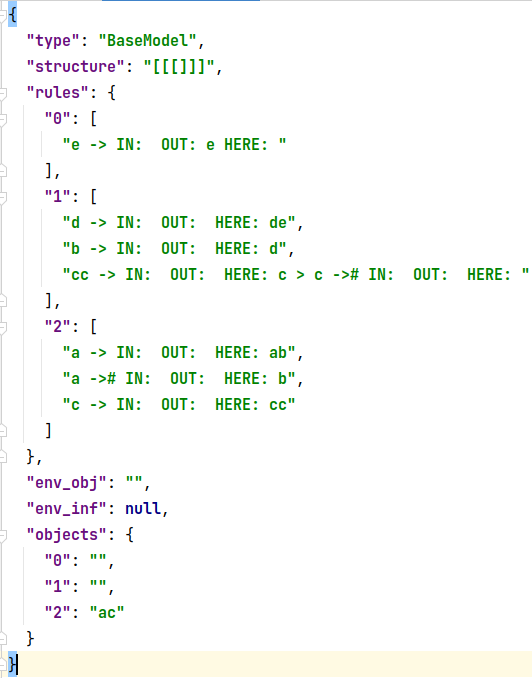
\includegraphics{saved_json_base.png}}
	\caption{Egy alapmodellbeli membránrendszerhez tartozó \textit{JSON} szótár}
	\label{fig:save_model_base}
\end{figure}

A \textit{JSON} szótár részletes tartalmát a \ref{fig:save_model_base} ábra szemlélteti:
\begin{itemize}
\item \verb|type|: A membránrendszer típusa.
\item \verb|structure|: A membránrendszerhez tartozó struktúrát reprezentáló sztring (az esetleges objektumok elhagyásával).
\item \verb|rules|: A membránrendszer szabályait tartalmazó szótár. A kulcsok a régió egyedi azonosítói, az értékek pedig a szabályok sztring reprezentációjából álló listák.
\item \verb|env_obj|: A környezetben nem korlátlanul rendelkezésre álló objektumokból álló multihalmaz sztring reprezentációja.
\item \verb|env_inf|:  A környezetben korlátlanul rendelkezésre álló objektumokból álló lista.
\item \verb|objects|: A membránrendszer objektumait tartalmazó szótár. A kulcsok a régió egyedi azonosítói, az értékek pedig az adott régióhoz tartozó objektumokból álló multihalmaz sztring reprezentációi. 
\end{itemize}

Ekkor a \textit{JSON} szótár minden információt tartalmaz mindkét támogatott típus újbóli betöltéséhez.

\subsection{Betöltés}

A betöltés az előző alfejezetben említett \verb|JSON| szótárat fogja igénybe venni. Miután a felhasználó kiválasztotta a betölteni kívánt membránrendszert tartalmazó fájlt, meghívásra kerül a \verb|MembraneSystem| ősosztályban implementált \verb|load()| metódus, amely a betöltés után a szótárban található \verb|"structure"| kulcshoz tartozó sztringgel meghívja a \verb|create_model_from_str()| metódust. Ez a metódus pedig azon osztály implementációjával lesz meghívva (az ősztály definiálja, de nem implementálja), amely típusnak a neve található a \verb|"type"| értéknél. Így a dinamikus típusosság következtében mindig a megfelelő típusú membránrendszer lesz példányosítva. Ekkor még sem szabályt sem objektumokat nem fog tartalmazni, ám a szótárban található többi információ segítségével ez is elvégezhető. Ehhez azonban fontos, hogy a szabályok és objektumok sztring reprezentációját képes legyen mindegyik membránrendszerből leszármazott típus átalakítani a megfelelő \verb|Rule| vagy \verb|MultiSet| típusra. Ezen paraméterek feldolgozása után előáll a kívánt konfigurációjú membránrendszer. A felhasználó által megadott bemenet feldolgozásáról a következő alfejezetben esik részletesen szó.

\subsection{Felhasználói bemenet feldolgozása}

Az alkalmazás használata során számos helyen a felhasználó által megadott input segítségével hajt végre módosításokat a membránrendszeren. A felhasználó szöveges módon adja meg a régiók objektumait és szabályait, illetve a membránrendszer struktúráját is egy sztring segítségével teheti meg. Ezen interakciók aktualizálásához szükség van olyan metódusokra, amelyek ezt a sztring reprezentációt a modell architektúrájában a ténylegesen felhasználható formára konvertálják.

\subsubsection{Struktúra megadása}
A struktúra megadásánál kihagyhatatlan a megadott bemenet helyességének ellenőrzése.
Ennek feltételei:
\begin{itemize}
\item A bemenetben a zárójelezésre használt szimbólumok és a szimport-antiport rendszerek esetében kimeneti régió jelzésére használt \verb|#| karakteren kívül csak a szóköz és az angol ábécé kisbetűi szerepelhetnek.
\item A megadott kifejezésnek meg kell felelnie a helyes zárójelezés szabályainak. Ennek eldöntéséhez verem adatszerkezetet használ az algoritmus.
\end{itemize}

\lstset{caption={A helyes zárójelezést eldöntő algoritmus}, label=src:valid_parentheses}
\begin{lstlisting}[language={Python}]
def is_valid_parentheses(cls, m_str):
	open_paren = set(['(', '{', '['])
	close_paren = set([')', '}', ']'])
	stack = []
	pairs = {'}': '{', ')': '(', ']': '['}

	for c in m_str:
		if c in close_paren:
			if not stack:
				return False
		elif pairs[c] != stack.pop():
				return False
		else:
			continue
		if c not in open_paren.union(close_paren):
			continue
		if c in open_paren:
                stack.append(c)
	if not stack:
		return True
	else:
		return False
\end{lstlisting}

Ha a függvény igaz értékkel tér vissza, akkor létrehozható a struktúrához tartozó membránrendszer a \verb|create_model_from_str()| metódus meghívásával (a megfelelő osztály implementációja szerint). 

Szimport antiport rendszerek esetében a legkülső régióhoz tartozó zárójelpáron kívülre írhatóak a korlátlanul rendelkezésre álló objektumok. Megengedett a karakterek ismétlődése, hiszen ilyenkor  az objektum többszörös jelenléte nem befolyásolja a környezetet viselkedését. A szóköz karakter itt is megengedett és nem kerül figyelembe vételre.

\subsubsection{Objektumok megadása}
Az objektumok megadása történhet a struktúra megadásánál és a már létrehozott membránrendszer szerkesztésénél is. A struktúra megadásánál a megfelelő régióhoz tartozó zárójelpár között kell szerepeljenek azok az objektumok, amely a régió kezdeti tartalmát fogják alkotni. A membránrendszer szerkesztésénél a vizuális felületen a szerkesztendő régióra való dupla kattintás után megjelenő felső szövegdobozban kerülnek rögzítésre a módosított objektumok. Mindkét esetben a következő feltételek érvényesek:

\begin{itemize}
\item A bemenetben csak szóköz és az angol ábécé kisbetűjei szerepelhetnek.
\item A szóköz karakterek nem kerülnek figyelembe vételre az objektumok feldolgozásánál.
\end{itemize}

A bemeneti sztring feldolgozásáért a \verb|MultiSet| osztály osztályszintű \verb|string_to_multiset()| metódusa felel, amely karakterenként dolgozza fel a bemenetet és a nem szóköz karaktereket az eredmény multihalmazhoz a \verb|add_object()| metódus segítségével adja hozzá.

\subsubsection{Szabályok megadása}

A szabályok megadása egyedül már a létrehozott membránrendszer szerkesztésekor támogatott. A szabályok alakja és viselkedése is eltér az egyes membránrendszer típusok esetén, ezért ezek különböző módszerekkel kerülnek feldolgozásra.

Alapmodell esetén a következőknek kell megfelelni a bemeneti szövegnek:
\begin{itemize}
\item  A szabályok alakja: \\
\begin{small}
\verb|"szükséges ->(#) IN: bevándorló OUT: kivándorló HERE: helyben_keletkező"|
\end{small} 
\item Az objektumokat reprezentáló részsztringben tetszőleges számban szereplhet szóköz karakter, azon kívül csak az angol ábécé kisbetűi szerepelhetnek.
\item A szabály végbemeneteléhez szükséges objektumok száma legalább egy kell legyen
\item Ha az opcionális \verb|#| karakter szerepel a megfelelő pozícióban, akkor a megadott szabály feloldódást fog eredményezni
\item Ha egy sorban szerepel két, az előbbi formátumnak megfelelő, \verb|>| szimbólummal elválasztott szabály, olyankor a megadott páros egy \verb|PriorityRule| típusú objektumként lesz értelmezve. 
\end{itemize}

A szabály megfelelő formátumának ellenőrzését egy reguláris kifejezés végzi, amely egyben azt is ellenőrzi, hogy a szabály bal oldala legalább egy objektumból áll.

Szimport antiport rendszerek esetén a három szabálytípusnak megfelelően három formátum is támogatott a feldolgozás során:
\begin{compactenum}
\item \verb|"IN: importált_objektumok"|
\item \verb|"OUT: exportált_objektumok"|
\item 
\begin{small}
\verb|"IN: importált_objektumok OUT: exportált_objektumok" | vagy \\ \verb|"OUT: exportált_objektumok IN: importált_objektumok "|
\end{small}
\end{compactenum}

Itt is elmondható, hogy az objektumokat reprezentáló részsztringben tetszőleges számban szereplhet szóköz karakter, azon kívül csak az angol ábécé kisbetűi szerepelhetnek.

A helyes formátummal megadott szabályok feldolgozásáért a \verb|MembraneSystem| osztályban definiált \verb|parse_rule()| metódus felelős, amely a különböző modelltípusoknál más implementációval rendelkezik. Egy membránrendszer betöltésekor is ez a metódus alakítja át a szöveges reprezentációt a megfelelő \verb|Rule| altípusú példánnyá.

\section{Nézet}

A membránrendszerek vizuális megjelenítését a grafikus felület biztosítja, amely a felhasználóval való kommunikáció 
során bekövetkezett eseményekről tájékoztatja a modellt.

A tervezés során fontos szempont a \textit{Qt} keretrendszer grafikus eszközei által nyújtott lehetőségek feltárása, hiszen a membránrendszer vizualizálásának megvalósításához egy olyan vászonra van szükség, amely egy tetszőleges membránstruktúrához tartozó sejtszerű ábrát tud megjeleníteni, amelyben az egyes régiók mozgathatóak. Maga a felület a \verb|QGraphicsScene| és a \verb|QGraphicsView| osztályok közös felhasználásával valósítható meg, ahol az előbbi törődik a "vásznon" található objektumok eltárolásával és manipulálásával, az utóbbi pedig mindezek megjelenítésével. 
A membránrendszer egyes régióinak kirajzolásához és a bennük található objektumok és szabályok vizuális megjelenítéséért a \verb|QGraphicsRectItem| osztályból leszármaztatott \verb|RegionView| osztály felelős. Mindezen funkciók és megjelenített régiók összefogására a \verb|MembraneSimulator| osztály hivatott, amely a modell felől érkező szignálokra eseménykezelő metódusokkal feliratkozik. Ez az osztály az egyes régiókhoz tartozó \verb|RegionView| példányokat a modellben látottakhoz hasonlóan egy szótárban tárolja, ahol az egyes objektumokhoz tartozó kulcsot a modell adott régiójának egyedi azonosítója jelenti. Így biztosítható az, hogy a nézet oldalán egyértelműen beazonosítható egy régió és a hozzá tartozó megjelenítés. 

A szofver főablakát tartalmazó \verb|MainWindow| osztály a \verb|QMainWindow| osztályból származik le, így megörökli az alkalmazás számára hasznos menüsor és státuszsor felhelyezésének lehetőségét. A felhasználóbarát és könnyen átlátható felület elérésének érdekében az adatok bekérése dialógusablakok segítségével történik, amelyekben a megadott bemenet ellenőrzésre kerül. Hiba esetén a felhasználó figyelmeztetésére egy üzenetablak jelenik minden esetben.

\begin{figure}[H]
\advance\leftskip-3cm
	\scalebox{0.6}[0.6]{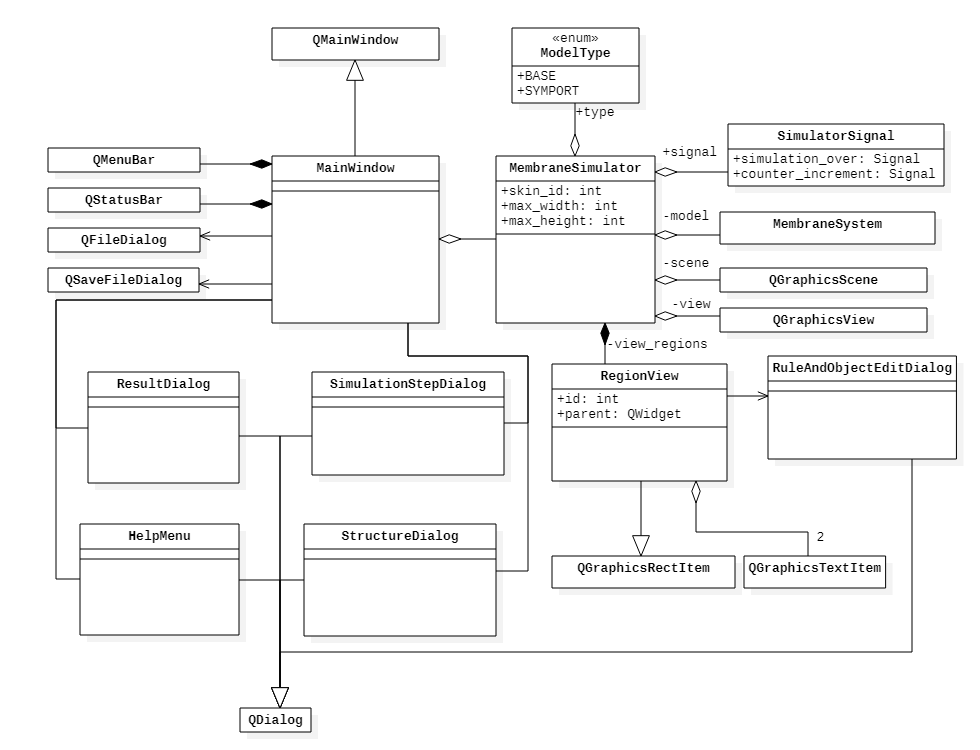
\includegraphics{uml_view_no_methods.png}}
	\caption{A szoftver nézetének osztály diagramja}
	\label{fig:save_model_base}
\end{figure}

\subsection{Főablak}

Az alkalmazás főablaka tartalmazza a felhasználóval való interakció megteremtéséért felelős \verb|QAction| típusú objektumokat, amelyek a menüsorban találhatóak. Ezen funkciók almenükre vannak osztva, a megfelelő gombra való kattintással vagy a funkcióhoz tartozó billentyűzetkombináció lenyomásával kezdeményezhető a dialógusablak megnyitása. Ezen dialógus ablakok közé tartoznak a két típusú membránrendszer struktúrájának megadását, illetve a mentés-betöltés funkciókat ellátó ablakok. Emellett ha már egy membránrendszer betöltésre került, akkor a főablak alján egy \verb|QStatusBar| is megjelenik, amely két gombot tartalmaz a szimuláció két futtatási módjához, illetve a lépések számát megjelenítő \verb|QLabel| objektumot.
A menüsor helyet ad a súgó megjelenítését előidéző \verb|QAction| objektumnak is.

\begin{figure}[H]
\centering
	\scalebox{0.6}[0.6]{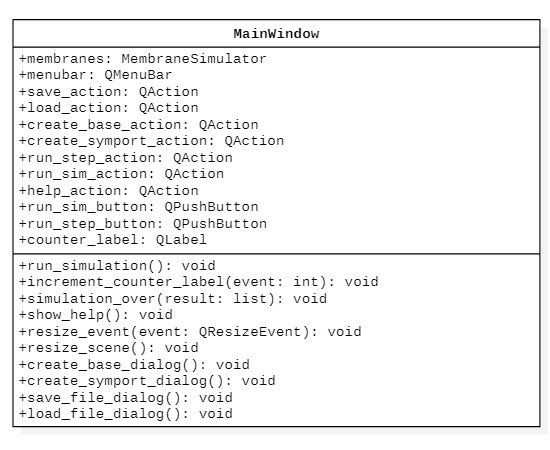
\includegraphics{uml_main_window.png}}
	\caption{Az alkalmazás főablakának osztály diagramja}
	\label{fig:uml_mainwindow}
\end{figure}

A főablak legfontosabb komponense a központi \textit{widget}-ként funkcionáló (a membránrendszer szimulálásáért felelős)  \verb|MembraneSimulator| osztály \verb|QGraphicsView| típusú adattagja, amely a modellben található membránrendszer vizualizációját jeleníti meg.

\subsection{Membránrendszer szimulátor osztály}

A  \verb|MembraneSimulator| osztály az üzleti logikát magába foglaló \verb|MembraneSystem| osztályt és annak vizualizálásához szükséges objektumokat aggregálja. Ez az osztály felelős a modell által kommunikált szignálok feldolgozásáért, illetve a felhasználó által megadott utasítások továbbításáért. A dialógusablakok biztosítják azt, hogy a felhasználó csak a megfelelő formátumú input leírásával tud a modell számára szánt változtatásokat kezdeményezni. A \verb|MembraneSimulator| osztály letárolja a jelenleg szimulálás alatt álló membránrendszer típusát, a legkülső régiójának egyedi azonosítóját (erre az alakzat kirajzolása miatt van szükség), illetve a megrajzolt sejtszerkezet által elfoglalható maximális méretet.

\begin{figure}[H]
\centering
	\scalebox{0.5}[0.5]{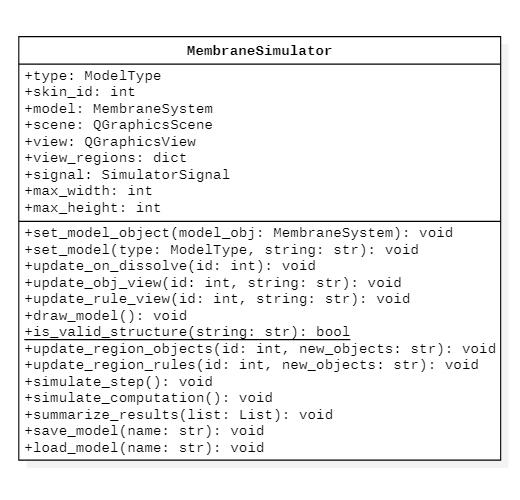
\includegraphics{uml_simulator.png}}
	\caption{Membránrendszer szimulátor osztály diagramja}
	\label{fig:uml_simulator}
\end{figure}

A \verb|MembraneSimulator| osztály az általa aggregált \verb|QGraphicsScene| és \verb|QGraphicsView| objektumok segítségével jeleníti meg a membránrendszert, amelyben minden régió a hozzá tartozó \verb|RegionView| osztálybeli objektum megrajzolásával kerül megjelenítésre. 

Az osztály feliratkozik a \verb|MembraneSystem| által kibocsájtott szignálokra, ezáltal képes az egyes régiókban az objektumok és szabályok új állapotát befrissíteni. Fontos ilyen szignál még a \verb|region_dissolved()|, amely fellépésekor paraméterként hordozza a felbomlás alatt lévő régió sorszámát. Ilyenkor a hozzá tartozó alakzatot törlésre kerül a  grafikus felületről, illetve a gyerek régiók szülő referenciája is megfelelően módosul. 

A felhasználó által megadott, illetve a szűrő által validnak vélt sztringeket az \verb|update_region_objects()| és \verb|update_region_rules()| metódusok továbbítják a modell felé, amely feldolgozza a sztringeket és a megfelelő módosításokat hajtja végre saját állapotában.

Ezen osztály feladata még a párhuzamos számítások indítása esetén az eredmények összegzése, azaz gyakoriságok alapján rendezni a különböző eredményeket, majd egy szignál segítségével ezt továbbítani a főablaknak.

\subsubsection{Régiók vizualizálása}

A teljes membránstruktúra megrajzolásáért a \verb|MembraneSimulator| osztály \verb|draw_model()| metódusa felelős. Az osztály rendelkezik a teljes rendszer számára biztosítható maximális szélességet és maximális magasságot meghatározó adattagokkal, amelyek a megrajzolt alakzat teljes láthatóságát garantálják. Ezek után kezdődhet a régiók legenerálása, amely a következő algoritmust követi:

\begin{algorithm}[H]
\caption{A régiók megrajzolására használt algoritmus}
\label{alg:draw_model}
\begin{algorithmic}[1] % sorszámok megjelenítése minden n. sor előtt, most n = 1
\State Legyen $genChildList := [rootNode]$
\State Generáljuk le a legkülső régióhoz tartozó alakzatot
\While{( $genChildList \neq []$ )}
	\State $currentNode := genChildList.pop()$
	\State Generáljuk le a $currentNode$ régiót
	\State $numOfChildren := currentNode.getNumOfChildren()$
	\If{$numOfChildren \neq 0$}
		\For{$i=1,\ldots,numOfChildren$}
		\State $genChildList = genChildList + currentNode.children[i]$
		\EndFor
	\EndIf
\EndWhile
\end{algorithmic}
\end{algorithm}

Az algoritmus garantálja, hogy egy gyerek régió csakis a szülő régió legenerálása után kerül feldolgozásra, illetve, hogy minden régió pontosan egyszer kerül kiterjesztésre. Ez az információ fontos ugyanis akkor, amikor a régióhoz megrajzolt lekerekített oldalú téglalap mérete kerül meghatározásra.  Egy régió méretét az határozza meg, hogy hány testvére van, illetve, hogy a membránstruktúra fa szerkezetében milyen mélységben helyezkedik el.

Egy adott régió kirajzolása pedig az általa határolt membrán, illetve a benne található objektumok és szabályok megjelenítésével történik. Miután a \verb|draw_model()| metódus kiszámolta a kialakuló régió méretét, ezt átadja a \verb|RegionView| típusú objektum konstruktorának paraméterként. Ekkor a \verb|RegionView| \verb|draw()| metódusának feladata magát a lekerekített oldalú téglalapot megrajzolni, illetve vízszintesen középre zárva a benne található objektumok és szabályok megjelenítését szolgáló \verb|QGraphicsTextItem| típusú objektumokat létrehoznia. Ezek automatikusan megjelenítik a bennük található szöveget.

\subsection{Dialógusablakok}

Az alkalmazás számos dialógusablakot biztosít a felhasználó számára, amelyen keresztül manipulálni tudja a szimulált membránrendszer belső állapotát. Ezen dialógusablakok nagyrészt egy funkció ellátásra szolgálnak.

\subsubsection{Membránstruktúra}

\begin{figure}[H]
\centering
	\scalebox{0.8}[0.8]{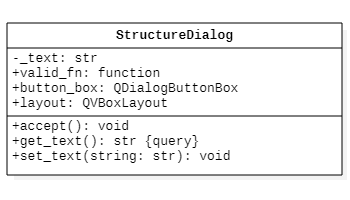
\includegraphics{uml_structure_dialog.png}}
	\caption{Membránstruktúra megadásához használt dialógusablak diagramja}
	\label{fig:uml_structure}
\end{figure}

A dialógusablakon egy szövegdoboz rögzíti a felhasználó által megadott struktúrát, amely a \verb|MembraneSystem| ősosztályban definiált \verb|is_valid_parentheses()| metódus segítségével kerül validálásra. A szövegdoboz mellett még egy \verb|QDialogButtonBox| típusú osztály biztosítja az ablak elfogadására és bezárása használt gombokat. Ha a felhasználó a \verb|Cancel| gombra kattint, akkor a dialógusablakba írt tartalom nem kerül feldolgozásra. A dialógusablak elrendezése a \verb|QVBoxLayout| osztály segítségével kerül beállításra. A dialógusablak bezárása után a begépelt szöveg a \verb|text| adattag getter metódusán keresztül érhető el.

\subsubsection{Használati útmutatót megjelenítő dialógusablak}

A dialógusablak elrendezését hasonlóan az előző dialógusablakhoz a \verb|QVBoxLayout| osztály alakítja ki, illetve a dialógusablak elrejtéséhez a \verb|QDialogButtonBox| osztályt használja. Az ablakban megjelenített szöveg a \verb|help_md| \verb|QTextEdit| típusú változó segítségével \textit{Markdown} formázással jelenik meg.

\subsubsection{A párhuzamos számítások számát beállító dialógusablak}

A párhuzamos számítások számát beállító dialógusablak a korábbiakban ismertett technikákat használja az elrendezésre és a dialógusablak elfogadására, illetve elutasítására. A számítások számának beállítására a \verb|QSpinBox| típusú \verb|spin_box| változót aggregálja, amelynek értékét a felhasználó \verb|OK| gombra kattintása után a \verb|get_number()| metódus segítségével lehet lekérdezni.

\subsubsection{Egy régió szerkesztéséért felelős dialógusablak} 

Mivel ez a dialógusablak mindig egy adott régió tartalmához kötődik, ezért megjelenítése is ahhoz az egyhez kell kapcsolódjon. Így az ilyen dialógusablakok megjelenítését a szerkeszteni kívánt régió által lefedett területre való dupla kattintással lehet kezdményezni. Ezen dialógusablak két szövegdobozt nyújt a felhasználó bemenetének fogadására, az egyik az objektumok, a másik pedig a szabályok rögzítéséért felelős. Miután a felhasználó a \verb|QDialogButtonBox| típusó dobozban az \verb|OK| gombot választja, a megadott bemenet ellenőrzésre kerül. Az objektumok esetén elegendő egy reguláris kifejezéssel szűrni, hogy a megadott sztring kizárólag csak szóközt és/vagy az angol ábécé kisbetűit tartalmazza. A szabályok esetében viszont a bemenetet soronként kell ellenőrizni. Ilyenkor az üres sorokat figyelmen kívül hagyva a dialógusablak paraméterként megkapott \verb|is_valid_rule()| metódus segítségével ellenőrzi a szabályok helyességét. Ha legalább egy szabály vagy az objektumok formátuma nem megfelelő, akkor egy \verb|QMessageBox| típusú ablak jelenik meg a felhasználó értesítésére. 

\newpage
\section{Tesztelési terv és eredmények}

A program egyes komponensei egységtesztek segítségével kerülnek ellenőrzésre. Ezen egységtesztek az egyes metódusok esetében a teljes lefedettségre törekednek, ahol különös figyelmet kapnak a szélsőséges esetek és a hibás viselkedés lekezelése.

\subsection{Multihalmaz osztály tesztelése}

\begin{table}[H]
	\centering
	\begin{tabular}{ | m{0.75\textwidth} | m{0.15\textwidth} | }
		\hline
		\textbf{Tesztesetek leírása} & \textbf{Teszteset eredménye} \\
		\hline \hline
		Üres multihalmazra meghívott \verb|is_empty()| metódus igaz értékkel tér vissza & Sikeres \\
		\hline
	Nemüres multihalmazra meghívott \verb|is_empty()| metódus hamis értékkel tér vissza & Sikeres \\
		\hline
		
		A multihalmazhoz egyetlen elemet adva eggyel nő meg a mérete &  Sikeres \\
		\hline
		
		A multihalmazhoz egynél nagyobb multiplicitással rendelkező objektum hozzáadásánál pontosan annak elemszámmal nő meg a multihalmaz mérete &  Sikeres \\
		\hline
		A multihalmazból egy elemet törölve eggyel csökken annak mérete &  Sikeres \\
		\hline
		
		A multihalmazból egy meglévő objektum multiplicitásánál kevesebb elemet törölve a megfelelő mértékben csökken mérete &  Sikeres \\
		\hline
		A multihalmazból egy meglévő objektum multiplicitásánál több elemet törlése esetén \verb|NotEnoughObjectsException| kivétel kerül kiváltásra &  Sikeres \\
		\hline
				A multihalmazból egy nem benne szereplő objektum törlésének próbálkozása esetén \verb|ObjectNotFoundException| kivétel kerül kiváltásra &  Sikeres \\
		\hline
		
		Egy multihalmazból néhány objektum (teljes vagy részleges multiplicitással való) törlésével  kapott multihalmaz részhalmaza az eredetinek &  Sikeres \\
		\hline
		
		Egy multihalmazhoz néhány objektum hozzáadásával kapott multihalmaz nem részhalmaza az eredetinek &  Sikeres \\
		\hline
		
				Egy multihalmazhozból egy annak nem részhalmazát jelentő multihalmaz kivonása \verb|InvalidOperationException| kiváltását eredményezi &  Sikeres \\
		\hline
		
		
		Egy multihalmaz inicializálásakor negatív multiplicitású objektum esetén \verb|AssertionError| kerül kiváltásra &  Sikeres \\
		\hline
		
		Egy multihalmazra meghívott \verb|multiplicity()| metódus visszatérési értéke megegyezik a paraméterként kapott objektum multihalmazbeli számosságával &  Sikeres \\
		\hline
		
	\end{tabular}
	\caption{A tesztesetek leírása}
	\label{tab:test_cases_multiset}
\end{table}

\subsection{Membránstruktúra tesztelése}

\begin{table}[H]
	\centering
	\begin{tabular}{ | m{0.75\textwidth} | m{0.15\textwidth} | }
		\hline
		\textbf{Tesztesetek leírása} & \textbf{Teszteset eredménye} \\
		\hline \hline
		Egy csúcs létrehozása után az \verb|is_leaf()| metódus igaz értékkel tér vissza & Sikeres \\
		\hline
		Egy csúcs gyerekeihez való beszúrás után az \verb|is_leaf()| metódus hamis értékkel tér vissza & Sikeres \\
		\hline
		
		A membránstruktúrában a skin régiónak nincs szülője & Sikeres \\
		\hline
		
		A membránstruktúrában egy csúcs törlése esetén annak gyerekeinek szülő lekérdezése az eredeti csúcs szülőjével tér vissza & Sikeres \\
		\hline
	A membránstruktúrában egy csúcs törlése esetén szülőjének gyerekeinek száma eggyel kevesebb fog nőni a törlés után, mint amennyi gyereke volt a törölt csúcsnak & Sikeres \\
		\hline
		
			A membránstruktúrában egy csúcs gyerekeinek számának lekérdezése a \verb|children| listában tárolt csúcsok számával egyezik meg & Sikeres \\
		\hline
	\end{tabular}
	\caption{A tesztesetek leírása}
	\label{tab:test_cases_structure}
\end{table}

\subsection{Szabályok tesztelése}


\begin{table}[H]
	\centering
	\begin{tabular}{ | m{0.75\textwidth} | m{0.15\textwidth} | }
		\hline
		\textbf{Tesztesetek leírása} & \textbf{Teszteset eredménye} \\
		\hline \hline
		Egy alapmodellbeli szabály súlya megegyezik a bal oldalán található objektumok számával & Sikeres \\
		\hline
		
	  Egy prioritásos szabály nem alapmodellbeli szabályok megadása esetén \verb|InvalidTypeException| kivételt vált ki & Sikeres \\
		\hline
		
				Egy szimport-antiport rendszerhez tartozó antiport szabály súlya megegyezik az importált- és exportált objektumok elemszámának maximumával & Sikeres \\
		\hline
		
						Egy szimport-antiport rendszerhez tartozó szimport szabály súlya megegyezik az importált/exportált objektumok elemszámával & Sikeres \\
		\hline
	\end{tabular}
	\caption{A tesztesetek leírása}
	\label{tab:test_cases_rules}
\end{table}

\subsection{Feloldódás tesztelése}

\begin{table}[H]
	\centering
	\begin{tabular}{ | m{0.75\textwidth} | m{0.15\textwidth} | }
		\hline
		\textbf{Tesztesetek leírása} & \textbf{Teszteset eredménye} \\
		\hline \hline
		Ha egy felbomló régió egy gyerek régióval rendelkezik, akkor felbomlás után a felbomló régió szülője tartalmazni fogja a felbomlott régióban található objektumokat és a felbomlott régió egyetlen gyerekét & Sikeres \\
		\hline
		Ha egy felbomló régió több gyerek régióval rendelkezik, akkor felbomlás után a felbomló régió szülője tartalmazni fogja a felbomlott régióban található objektumokat és a felbomlott régió összes gyerekét & Sikeres \\
		\hline
		Ha a feloldódás a legkülső régióban kerül kezdeményezésre, akkor nem kerül meghívásra a \verb|dissolve_region()| metódus & Sikeres \\
		\hline
		
		Ha egyszerre bomlik egy szülő-gyerek pár, akkor az eredeti szülő szülője örökli meg mindkét bomló régió objektumait és a bomló gyerek régió összes gyerekét & Sikeres \\
		\hline
	\end{tabular}
	\caption{A tesztesetek leírása}
	\label{tab:test_cases_dissolve}
\end{table}


\subsection{Mentés és betöltés tesztelése}
\begin{table}[H]
	\centering
	\begin{tabular}{ | m{0.75\textwidth} | m{0.15\textwidth} | }
		\hline
		\textbf{Tesztesetek leírása} & \textbf{Teszteset eredménye} \\
		\hline \hline
		Egy \verb|save_model()| metódus segítségével lementett membránrendszerhez tartozó \textit{JSON} fájl régiónként a megfelelő objektumok és szabályok szöveges reprezentációját tartalmazza & Sikeres \\
		\hline
		Egy \verb|save_model()| metódus segítségével lementett membránrendszerhez tartozó \textit{JSON} fájl a membránrendszer struktúráját helyesen reprezentáló sztringet tartalmazza  & Sikeres \\
		\hline
		Egy \verb|save_model()| metódus segítségével lementett membránrendszerhez tartozó \textit{JSON} fájl a membránrendszer típusának nevét tartalmazza & Sikeres \\
		\hline
			Egy \verb|save_model()| metódus segítségével lementett membránrendszer \verb|load_model()| metódussal történő betöltése esetén visszakapjuk az eredeti membránrendszer konfigurációját & Sikeres \\
		\hline
		Egy \verb|save_model()| metódus segítségével lementett membránrendszer \verb|load_model()| metódussal történő betöltése után történő módosítások mentése esetén a lementett \textit{JSON} fájl is megfelelő módon változik meg & Sikeres \\
		\hline
	\end{tabular}
	\caption{A tesztesetek leírása}
	\label{tab:test_cases_save_and_load}
\end{table}

\subsection{Felhasználói bemenetet feldolgozó komponensek tesztelése}
\begin{table}[H]
	\centering
	\begin{tabular}{ | m{0.75\textwidth} | m{0.15\textwidth} | }
		\hline
		\textbf{Tesztesetek leírása} & \textbf{Teszteset eredménye} \\
		\hline \hline
		Nem megfelelő karaktert tartalmazó sztring esetén az \verb|is_valid_parentheses()| metódus hamis értékkel tér vissza & Sikeres \\
		\hline
		Átfedő zárójelpárokat tartalmazó sztring esetén az \verb|is_valid_parentheses()| metódus hamis értékkel tér vissza & Sikeres \\
		\hline
	Csak megengedett karakteret és helyes zárójelpárokat tartalmazó sztring esetén az \verb|is_valid_parentheses()| metódus igaz értékkel tér vissza & Sikeres \\
		\hline
		A   \verb|create_model_from_str()| metódus a megfelelő membránstruktúrával rendelkező membrárendszerrel tér vissza & Sikeres \\
				A   \verb|create_model_from_str()| metódus nem veszi figyelembe a szóköz karaktereket & Sikeres \\
		\hline
		A   \verb|create_model_from_str()| metódus által létrehozott membránrendszer az egyes régiókban a megadott sztringben szerepeltett objektumokat tartalmazza & Sikeres \\
		\hline
		Az   \verb|is_valid_rule()| metódus a szabályok szöveges reprezentációjánál részletezett reguláris kifejezésre illeszkedő sztringek esetén igaz értékkel tér vissza & Sikeres \\
		\hline
		Az   \verb|is_valid_rule()| metódus a szabályok szöveges reprezentációjánál részletezett reguláris kifejezésre nem illeszkedő sztringek esetén hamis értékkel tér vissza & Sikeres \\
		\hline
		Az   \verb|is_valid_rule()| a nem megengedett karaktereket tartalmazó sztringek esetén hamis értékkel tér vissza & Sikeres \\
		\hline
		
		Az \verb|is_valid_rule()| metódus által helyesnek vélt sztring feldolgozása után létrehozott szabály a sztringben szereplő összes objektumot tartalmazza & Sikeres \\
		\hline
				Alapmodell esetén ha az \verb|is_valid_rule()| metódus által helyesnek vélt sztring tartalmaz \verb|#| karaktert, akkor a  létrehozott szabály \verb|DissolvingRule| típusú & Sikeres \\
		\hline
		Az \verb|is_valid_rule()| metódus által helyesnek vélt sztring feldolgozása során a \verb|parse_rule()| metódus nem veszi figyelembe a szóköz karaktereket & Sikeres \\
		\hline

	\end{tabular}
	\caption{A tesztesetek leírása}
	\label{tab:test_cases_parse}
\end{table}

